\section{System Model and Problem}
\label{sec:model}

\subsection{System}
Fig.~\ref{fig:architecture} shows the system. IoT devices send one task in every time step. A task belongs to class $c \in \{1,\dots,K\}$ with probability $p_c$, independently of all other tasks. A task of class $c$ must finish within $L_c$ milliseconds. Each task is placed on one of $N$ edge nodes or on the cloud. Table~\ref{tab:symbols} lists all symbols.

\begin{figure}[t]
\centering
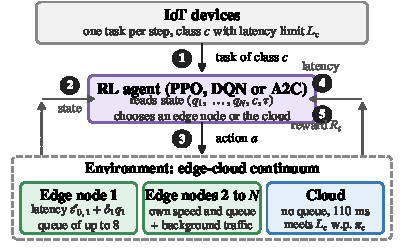
\includegraphics[width=0.95\columnwidth]{architecture.pdf}
\caption{Offloading loop. The numbers mark the steps of Section~\ref{sec:steps}.}
\label{fig:architecture}
\end{figure}

Edge node $i$ holds a queue of $q_i$ waiting tasks, with $0 \le q_i \le 8$. A task placed on edge node $i$ gets the latency
\begin{equation}
\ell = \ell_{0,i} + \delta_i\, q_i,
\label{eq:latency}
\end{equation}
where $\ell_{0,i}$ is the processing time of the node and $\delta_i$ is the extra wait for each task already in its queue. The latency is known when the task is placed, so a task on the edge meets its limit exactly when $\ell \le L_c$. The cloud has no queue. Its latency is 110\,ms on average, but the wide-area network makes it vary, so a cloud task of class $c$ meets its limit with a fixed probability $\pi_c$. In every system of this paper $\pi_c = 0$ for the most critical class, so the cloud never helps that class directly. Edge node $i$ finishes one task in a step with probability $d_i$. Other devices add background traffic that the agent does not control. Each background task joins the shortest edge queue. With $b$ background tasks per step on average, the offered edge load is
\begin{equation}
\rho = \frac{1 + b}{\sum_i d_i}.
\label{eq:load}
\end{equation}
All systems in this paper run at $\rho = 1$, so the edge can only keep up if some tasks go to the cloud and the classes compete for edge capacity. An episode has $T=200$ steps.

\begin{table}[t]
\caption{Symbols. Latencies in milliseconds.}
\label{tab:symbols}
\centering
\footnotesize
\setlength{\tabcolsep}{3pt}
\begin{tabular}{@{}l>{\raggedright\arraybackslash}p{6.2cm}@{}}
\toprule
Symbol & Meaning \\
\midrule
$N, K$ & number of edge nodes and of task classes \\
$c_t$ & class of the task at step $t$ \\
$p_c$ & share of tasks of class $c$ \\
$L_c$ & latency limit of class $c$ \\
$q_i$ & tasks waiting at edge node $i$, from 0 to 8 \\
$\ell_{0,i}, \delta_i$ & processing time of node $i$, wait per queued task \\
$d_i$ & chance that node $i$ finishes a task in a step \\
$\pi_c$ & chance that a cloud task of class $c$ meets its limit \\
$b$ & background tasks per step \\
$\rho$ & offered edge load, Eq.~\eqref{eq:load} \\
$T$, $\tau_t$ & steps per episode, share of the episode still to come \\
$w_c$ & miss penalty of class $c$ in the reward \\
$\bar w$ & miss penalty of the class-blind reward \\
$\beta, \kappa$ & reward for a met limit, cost of a cloud placement \\
$e_c$ & operator weight of a missed task of class $c$ \\
$v_c$ & share of tasks of class $c$ that miss the limit \\
$J$ & SLA cost per task, Eq.~\eqref{eq:cost} \\
\bottomrule
\end{tabular}
\end{table}

\subsection{Four Systems}
Table~\ref{tab:systems} lists the four systems. The nominal system is the one of the earlier conference version. It has two equal edge nodes and two classes, critical with a 50\,ms limit and analytics with a 90\,ms limit. An empty queue gives 30\,ms, which meets both limits. One waiting task gives 45\,ms, which still meets the critical limit. Two give 60\,ms, which misses the critical limit but meets the analytics limit. Background traffic arrives on a fixed schedule, one task every five steps, and the cloud never meets a limit. This makes the classes compete for the edge in the simplest possible way.

The three larger systems remove these simplifications. Their edge nodes differ in speed, background tasks arrive at random, and the cloud meets the analytics limit with some chance. Hetero3 has three edge nodes and two classes. Hetero3-3C has the same nodes and three classes with limits of 40, 70 and 110\,ms, which stand for control, interactive and analytics tasks. Large4-3C has four edge nodes and three classes. In the three-class systems the operator weights are 10, 4 and 1, and the cloud meets the 70\,ms limit with probability 0.2 and the 110\,ms limit with probability 0.6.

\begin{table}[t]
\caption{The four systems. All run at offered edge load $\rho=1$.}
\label{tab:systems}
\centering
\footnotesize
\setlength{\tabcolsep}{2.5pt}
\begin{tabular}{@{}lcccc@{}}
\toprule
 & Nominal & Hetero3 & Hetero3-3C & Large4-3C \\
\midrule
$N$, $K$ & 2, 2 & 3, 2 & 3, 3 & 4, 3 \\
$\ell_{0,i}$ & 30, 30 & 20, 30, 40 & 20, 30, 40 & 20, 25, 30, 40 \\
$\delta_i$ & 15, 15 & 10, 15, 20 & 10, 15, 20 & 10, 12, 15, 20 \\
$d_i$ & 0.6, 0.6 & 0.7, 0.6, 0.5 & 0.7, 0.6, 0.5 & 0.7, 0.6, 0.6, 0.5 \\
$b$, arrivals & 0.2, fixed & 0.8, random & 0.8, random & 1.4, random \\
$L_c$ & 50, 90 & 50, 90 & 40, 70, 110 & 40, 70, 110 \\
$p_c$ & 0.5, 0.5 & 0.5, 0.5 & 0.3, 0.3, 0.4 & 0.3, 0.3, 0.4 \\
$e_c$ & 10, 2 & 10, 2 & 10, 4, 1 & 10, 4, 1 \\
$\pi_c$ & 0, 0 & 0, 0.5 & 0, 0.2, 0.6 & 0, 0.2, 0.6 \\
States & 32,400 & 291,600 & 437,400 & 3,936,600 \\
\bottomrule
\end{tabular}
\end{table}

\subsection{Step by Step}
\label{sec:steps}
One step of the system runs as follows, numbered as in Fig.~\ref{fig:architecture}. (1) A device sends one task of class $c_t$. (2) The agent reads the state $s_t = (q_1,\dots,q_N, c_t, \tau_t)$, which holds the queue lengths, the class of the task and the share of the episode still to come, $\tau_t = 1 - t/T$. (3) The agent picks an action $a_t$, which is one of the edge nodes or the cloud. (4) The system computes the latency of the task from Eq.~\eqref{eq:latency}, or draws whether a cloud task meets its limit. If an edge node was chosen, the task joins its queue. Then the background tasks join the shortest queue, and each queue finishes one task with probability $d_i$. (5) The reward $R_t$ of Eq.~\eqref{eq:reward} is computed and used to update the agent. Then the next task arrives.

\subsection{Rewards}
With $m_t = 1$ if the task misses its limit and $m_t = 0$ otherwise, the reward of a step is
\begin{equation}
R_t = \beta\,(1-m_t) - w_{c_t}\, m_t - \kappa\,\mathbf{1}[a_t = \text{cloud}].
\label{eq:reward}
\end{equation}
A task that meets its limit earns $\beta = 1$. A task that misses costs $w_{c_t}$, the penalty of its class. The last term takes away $\kappa=0.1$ for every cloud placement, so the agent does not use the cloud without reason. Three choices of penalties are compared. The weighted reward uses the operator weights as penalties, $w_c = e_c$, which gives 10 and 2 in the nominal system. The class-blind (flat) reward uses one penalty for all classes,
\begin{equation}
\bar w = \sum_c p_c\, e_c ,
\label{eq:flat}
\end{equation}
which is 6 in the nominal system. Both rewards therefore have the same expected penalty for a missed task. The corrected reward is introduced in Section~\ref{sec:reward}. It has the same average penalty as the other two.

\subsection{Metrics and Objective}
For each class, $v_c$ is the share of tasks of that class that miss their limit. Edge use is the share of tasks placed on an edge node. One number is needed to rank policies. The SLA cost per task is
\begin{equation}
J = \sum_c p_c\, e_c\, v_c ,
\label{eq:cost}
\end{equation}
the expected operator weight of a missed task. In the nominal system $J = 5\,v_1 + v_2$, so a policy that misses every critical task and no analytics task has $J=5$. Because the weighted reward uses the operator weights as penalties, $J$ could seem to favor that reward by design. Section~\ref{sec:reward} shows that it does not favor it exactly, and the paper also reports the miss rate of every class, the full trade-off curve between the classes, and results for operator weights from 1:1 to 50:1.
